\chapter{Iteration 1: Design and Implementation}
\label{ch:iteration1}
% ============================================================

\section{Iteration Objectives}
Establish a reproducible zonal TSN simulation in which injected timing attacks
produce measurable, repeatable effects, and convert the resulting raw output into a
labelled protocol-native feature dataset. (Objectives O1--O3.)

\section{Selected Use Cases / Features}
UC-1 Configure and execute scenario; UC-2 Inject attack with ground truth;
UC-3 Extract feature dataset. Requirements FR-01 through FR-10.

\section{Design}
Iteration~1 realises layers L1 to L3 of the architecture in Figure~\ref{fig:arch},
together with the interface contracts IF-1 to IF-3 that join them. L1 is the
simulation layer, which produces raw clock-offset vectors. L2 is the extraction
layer, which converts those vectors into fixed windows and emits a feature row per
window per zone. L3 is the dataset layer, which holds the labelled feature table.
The detection and federation layers, L4 and L5, are deliberately out of scope for
this iteration.

The design decision that shapes the iteration is the boundary at IF-2, between
extraction and dataset. Everything above that boundary consumes a column contract
(Table~\ref{tab:schema}) rather than simulator output, so the detector never depends
on OMNeT++ data structures. This is what makes the pipeline replaceable by a captured
trace from real hardware in FYP-2 without changing the detection code, and it is the
reason extraction was completed and validated before any model was trained.

\section{Implementation}

\begin{figure}[htbp]
\centering
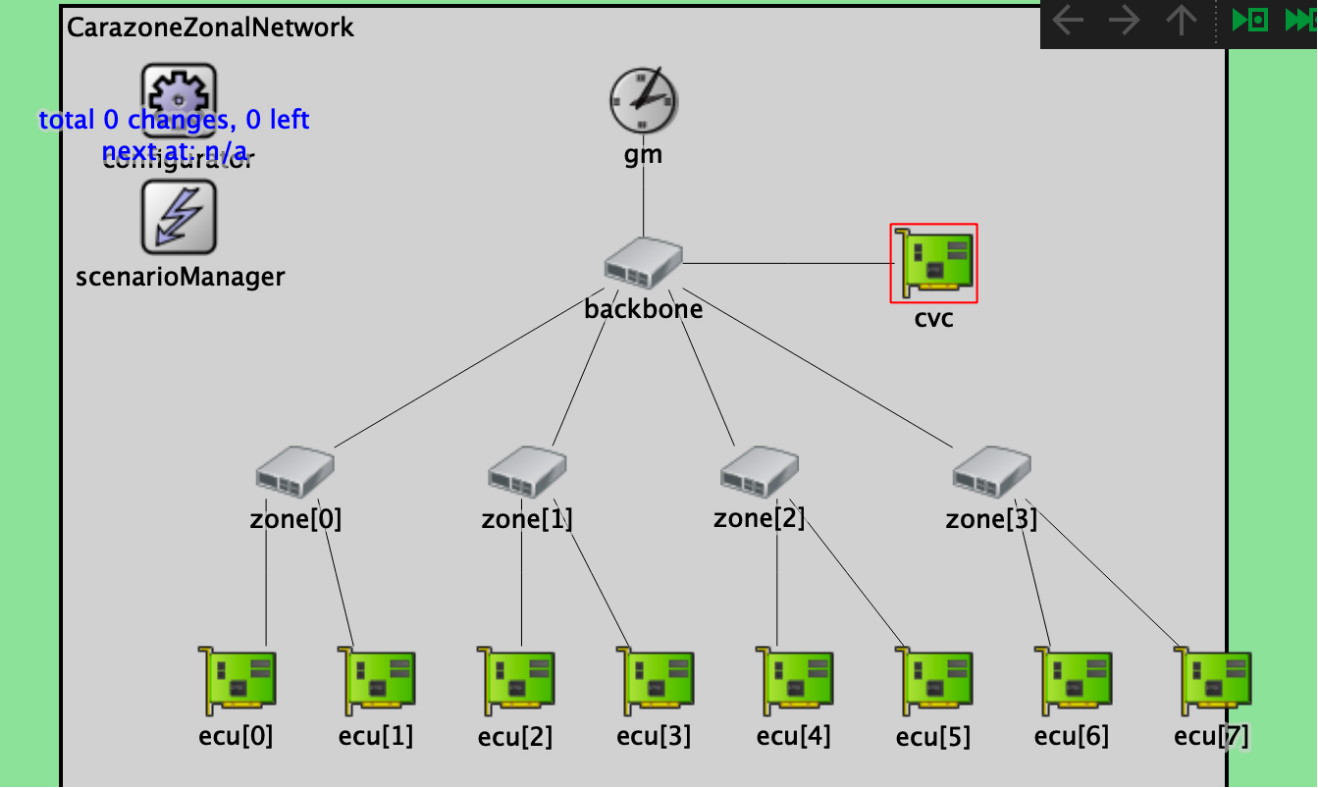
\includegraphics[width=0.95\textwidth]{basictopology.png}
\caption[Implemented four-zone tree topology]{Implemented zonal topology: grandmaster, backbone switch, four zone
controllers, eight endpoint ECUs and the central vehicle compute node.}
\label{fig:topology}
\end{figure}

The implemented topology comprises a grandmaster clock source, a backbone switch,
four zone controllers, eight endpoint ECUs (two per zone), and a central vehicle
compute node attached to the backbone. A configurator and a scenario manager handle
address assignment and timed attack events respectively. All time-aware nodes
participate in a single gPTP domain rooted at the grandmaster, giving a
synchronisation tree of depth three in which the four zone controllers are siblings.

\section{Completed Features / Module}
\begin{itemize}
  \item M1 Zonal Topology Simulation: complete
  \item M2 Attack Injection and Dataset: complete for three attack configurations
  \item M3 Feature Extraction Layer: complete, with DEF-01 open
\end{itemize}

\section{Technical Implementation Details}
\label{sec:technical-details}

\textbf{Environment.} OMNeT++ 6.4.0 with INET 4.7.0~\cite{inettsn}, on macOS (Apple Silicon).
The linked INET version is 4.7.0, which is the version whose
\texttt{driftRate} parameter is not declared \texttt{@mutable}. That property is the
reason the drift attack cannot be activated part-way through a run, and therefore the
reason the drift result in Section~\ref{sec:edge-cases} is reported as a limitation of the framework
rather than a finding about drift detectability.

\textbf{Key files.}
\begin{itemize}
  \item \texttt{CarazoneZonalNetwork.ned}: topology declaration: node types,
        links, and the submodule structure of the zonal network.
  \item \texttt{omnetpp.ini}: scenario configurations. Four named configurations
        are defined: \texttt{Benign}, \texttt{DelayAttack}, \texttt{DriftAttack} and
        \texttt{SyncStarvation}, together with clock drift parameters, gPTP settings
        and seed control.
  \item \texttt{carazone}: the built simulation executable.
  \item \texttt{extract\_features.py}: the feature extraction pipeline.
\end{itemize}

\textbf{Execution.} Scenarios are executed headlessly, selecting a configuration by
name:
\begin{verbatim}
./carazone -u Cmdenv -c Benign
./carazone -u Cmdenv -c DelayAttack
./carazone -u Cmdenv -c DriftAttack
./carazone -u Cmdenv -c SyncStarvation
\end{verbatim}
The graphical environment is used for topology inspection and single-run tracing:
\begin{verbatim}
./carazone -u Qtenv -c Benign -r 0
\end{verbatim}

\textbf{Feature extraction.} Extraction is invoked over a results directory:
\begin{verbatim}
python3 extract_features.py --results ../simulations/results --out features.csv
\end{verbatim}
Window length, stride and simulation limit are command-line parameters with defaults
of 0.25\,s, 0.125\,s and 10\,s respectively. The default window is twice the gPTP
synchronisation interval, so every window is expected to contain at least two
correction events under normal operation. The stride is half the window length,
giving 50\% overlap between consecutive windows. Dependencies are \texttt{pandas},
\texttt{numpy}, and \texttt{opp\_scavetool} from the OMNeT++ distribution on
\texttt{PATH}.

\textbf{Extraction pipeline.} The script proceeds in five stages:

\begin{enumerate}
  \item \texttt{run\_scavetool()} invokes \texttt{opp\_scavetool export -F CSV-R} over
        all \texttt{.vec} files in the results directory, producing one intermediate
        CSV. No scavetool filter expression is applied: match-expression syntax varies
        between tool versions and a rejected expression aborts the export, so the
        pipeline exports everything and filters in pandas. This trades a larger
        intermediate file for version robustness.
  \item \texttt{load\_export()} splits the export into a vector frame and a run-metadata
        frame. Vectors are filtered to names beginning \texttt{timeChanged}, excluding
        modules containing \texttt{underlyingClock} so that each node contributes its
        gPTP-corrected clock rather than its free-running oscillator. Run attributes
        and iteration variables are collected per run, which is how the configuration
        name and the victim zone are recovered.
  \item \texttt{node\_of()} and \texttt{zone\_of()} map a module path to a node and a
        node to a zone. A regular expression matches the node types
        \texttt{gm}, \texttt{cvc}, \texttt{backbone}, \texttt{zone[$i$]} and
        \texttt{ecu[$j$]}. Zone controllers map to their own index; ECUs map by integer
        division by \texttt{ECUS\_PER\_ZONE}. Nodes with no zone (grandmaster,
        backbone and central vehicle compute) are excluded, since they are not
        federated clients.
  \item \texttt{window\_features()} computes eight statistics per node per window. The
        zero-event case returns an explicit record with \texttt{n\_events = 0} rather
        than being discarded, because an empty window is itself the signature of
        synchronisation starvation. Offset is computed as \texttt{v - t} on the recorded
        series, giving error against the ideal timeline.
  \item \texttt{build()} iterates runs, then zones, then windows. For each window it
        computes per-node features, isolates the zone controller's own vector as the
        \texttt{ctrl\_} features, and aggregates mean and standard deviation across all
        nodes in the zone as the \texttt{zone\_} features. Labelling is delegated to
        \texttt{label\_for()}.
\end{enumerate}

\textbf{Labelling logic.} \texttt{label\_for(config, target\_zone, zone, w\_start)}
returns the benign class unless three conditions hold simultaneously: the run
configuration is an attack configuration; the zone under evaluation is the run's
designated victim zone, read from run metadata; and the attack is active over the
window, meaning either the window begins at or after \texttt{ATTACK\_START} or the
configuration is in \texttt{ALWAYS\_ON\_CONFIGS}. A bystander zone in an attack run is
therefore labelled benign, which is what makes zone attribution a learnable target.

\section{Algorithms and Technical Decisions}
\label{sec:algorithms}

\textbf{Windowing.} Raw per-node clock series are segmented into fixed-size
observation windows. The window size is a single global design parameter applied
consistently across all features so that one aligned feature vector is produced per
window per zone.

\textbf{Two-level feature construction.} Each window yields both the zone controller's
own statistics (\texttt{ctrl\_}) and the distribution of those statistics across all
nodes within the zone (\texttt{zone\_mean\_}, \texttt{zone\_std\_}). The controller is
the node that would host the detector in deployment, so its own view is preserved
separately; the within-zone spread captures whether a perturbation affects the
controller alone or the whole zone.

\textbf{Overlapping windows and split granularity.} The stride is half the window
length, so consecutive windows share half their samples. Adjacent windows are therefore
strongly correlated, and a random window-level train/test split would leak information
across the boundary. Splits are consequently formed at run and seed granularity
(integrity rule R3).

\textbf{Planned: cross-zone residual.} The implemented features are all computed within
a single zone. The design intent is that the discriminating feature is a residual
\emph{between} zones, taking a zone's controller offset minus the median across its
siblings in the synchronisation tree, because that is the quantity a generic traffic-feature
detector cannot construct. Computing it requires the observation window to be the outer
loop so that all zones are available simultaneously, which is a restructuring of
\texttt{build()} scheduled in Iteration~03.

\textbf{Consequence for attack coverage.} A sibling residual cancels common-mode
perturbation by construction, and is therefore insensitive to any effect that moves the
whole synchronisation tree together, including compromise at the grandmaster. This is
a structural property rather than a tuning deficiency, and it bounds the detection claim
to link-local timing integrity (Sections~\ref{sec:technical-challenges} and~\ref{sec:edge-cases}).

\section{Tools, Frameworks and Technologies}

\begin{longtable}{p{0.26\textwidth} p{0.16\textwidth} p{0.5\textwidth}}
\toprule
\textbf{Tool} & \textbf{Version} & \textbf{Purpose} \\
\midrule
\endhead
OMNeT++ & 6.4.0 & Discrete-event simulation kernel; Cmdenv for batch runs, Qtenv for
inspection \\
INET~\cite{inettsn} & 4.7.0 & TSN and gPTP protocol models, clock drift modelling \\
Python & 3.x & Feature extraction, dataset construction \\
Flower & not yet adopted & Federated learning framework; selected for Iteration~03, not yet introduced into the build \\
\bottomrule
\end{longtable}

\section{Demonstration Evidence}
\label{sec:demo-evidence}

\begin{figure}[htbp]
\centering
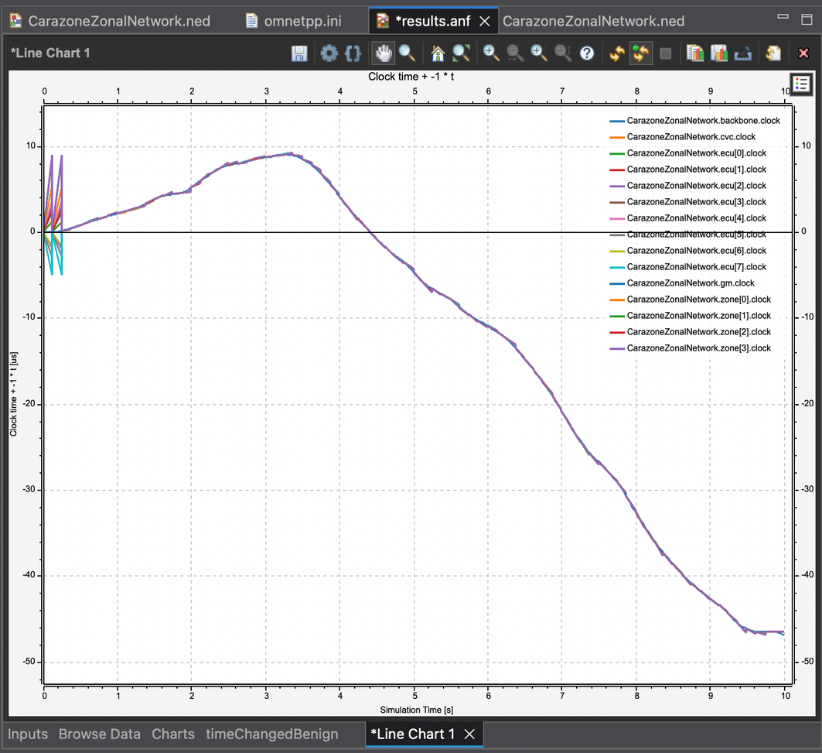
\includegraphics[width=0.92\textwidth]{benign.png}
\caption[Clock offset, benign run]{Clock offset against simulation time, benign run. All fourteen clocks
follow a single common trajectory; the individual traces are not separable at this
scale, which is the expected behaviour of a converged gPTP domain. The transient
before approximately $t = 0.5$~s is the synchronisation servo converging from its
initial state. That transient is the benign population discussed in
Section~\ref{sec:edge-cases}: it produces larger offset excursions than the attack does, which is why
a fixed threshold on offset alone cannot separate the two.}
\label{fig:offset-benign}
\end{figure}

\begin{figure}[htbp]
\centering
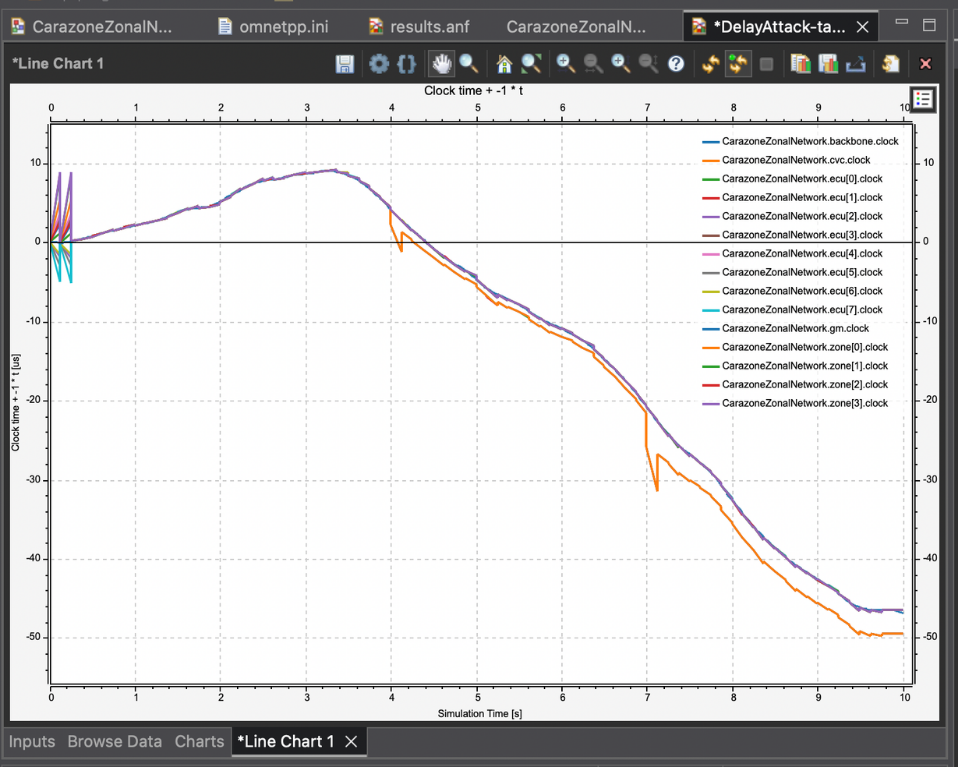
\includegraphics[width=0.92\textwidth]{attack.png}
\caption[Clock offset, delay attack on zone 0]{Clock offset against simulation time, delay attack on zone~0. The targeted
zone controller (orange) separates from the common trajectory at $t = 4$~s, the
attack onset, with a second visible step at $t = 7$~s; every other clock continues
to track the group. The attack is visible only as a disagreement between one zone
and its siblings, not as an absolute fault in the victim's own clock, which is the
observation the cross-zone sibling residual is built to capture
(Section~\ref{sec:algorithms}).}
\label{fig:offset-attack}
\end{figure}

Read together, Figures~\ref{fig:offset-benign} and~\ref{fig:offset-attack} are the
empirical basis of the sibling residual feature. In the benign run every clock
follows one trajectory. In the attacked run the targeted branch departs from that
trajectory at the attack onset while the siblings continue to track one another.
The quantity that changes between the two figures is not the victim's offset in
absolute terms, which continues to follow the same broad shape, but its
\emph{disagreement} with the zones beside it. That is precisely the quantity the
residual measures, and it is why a feature computed inside a single zone cannot see
this attack while a cross-zone comparison can.

\section{Iteration Outcome}
Iterations 01 and 02 met their exit criteria. The simulation produces repeatable,
seeded attack effects; the extraction pipeline produces a labelled dataset. One
defect (DEF-01) and one design limitation (zone symmetry) were identified and are
scheduled for correction before Iteration~03 modelling work begins.

% ============================================================